\PassOptionsToPackage{unicode=true}{hyperref} % options for packages loaded elsewhere
\PassOptionsToPackage{hyphens}{url}
%
\documentclass[]{article}
\usepackage{lmodern}
\usepackage{amssymb,amsmath}
\usepackage{ifxetex,ifluatex}
\usepackage{fixltx2e} % provides \textsubscript
\ifnum 0\ifxetex 1\fi\ifluatex 1\fi=0 % if pdftex
  \usepackage[T1]{fontenc}
  \usepackage[utf8]{inputenc}
  \usepackage{textcomp} % provides euro and other symbols
\else % if luatex or xelatex
  \usepackage{unicode-math}
  \defaultfontfeatures{Ligatures=TeX,Scale=MatchLowercase}
\fi
% use upquote if available, for straight quotes in verbatim environments
\IfFileExists{upquote.sty}{\usepackage{upquote}}{}
% use microtype if available
\IfFileExists{microtype.sty}{%
\usepackage[]{microtype}
\UseMicrotypeSet[protrusion]{basicmath} % disable protrusion for tt fonts
}{}
\IfFileExists{parskip.sty}{%
\usepackage{parskip}
}{% else
\setlength{\parindent}{0pt}
\setlength{\parskip}{6pt plus 2pt minus 1pt}
}
\usepackage{hyperref}
\hypersetup{
            pdftitle={Modelos no Supervisados},
            pdfauthor={Sebastian Jaremczuk},
            pdfborder={0 0 0},
            breaklinks=true}
\urlstyle{same}  % don't use monospace font for urls
\usepackage[margin=1in]{geometry}
\usepackage{listings}
\newcommand{\passthrough}[1]{#1}
\usepackage{graphicx,grffile}
\makeatletter
\def\maxwidth{\ifdim\Gin@nat@width>\linewidth\linewidth\else\Gin@nat@width\fi}
\def\maxheight{\ifdim\Gin@nat@height>\textheight\textheight\else\Gin@nat@height\fi}
\makeatother
% Scale images if necessary, so that they will not overflow the page
% margins by default, and it is still possible to overwrite the defaults
% using explicit options in \includegraphics[width, height, ...]{}
\setkeys{Gin}{width=\maxwidth,height=\maxheight,keepaspectratio}
\setlength{\emergencystretch}{3em}  % prevent overfull lines
\providecommand{\tightlist}{%
  \setlength{\itemsep}{0pt}\setlength{\parskip}{0pt}}
\setcounter{secnumdepth}{0}
% Redefines (sub)paragraphs to behave more like sections
\ifx\paragraph\undefined\else
\let\oldparagraph\paragraph
\renewcommand{\paragraph}[1]{\oldparagraph{#1}\mbox{}}
\fi
\ifx\subparagraph\undefined\else
\let\oldsubparagraph\subparagraph
\renewcommand{\subparagraph}[1]{\oldsubparagraph{#1}\mbox{}}
\fi

% set default figure placement to htbp
\makeatletter
\def\fps@figure{htbp}
\makeatother

\usepackage{booktabs}
\usepackage{longtable}
\usepackage{array}
\usepackage{multirow}
\usepackage{wrapfig}
\usepackage{float}
\usepackage{colortbl}
\usepackage{pdflscape}
\usepackage{tabu}
\usepackage{threeparttable}
\usepackage{threeparttablex}
\usepackage[normalem]{ulem}
\usepackage{makecell}
\usepackage{xcolor}

\title{Modelos no Supervisados}
\author{Sebastian Jaremczuk}
\date{2020-04-17}

\begin{document}
\maketitle

\hypertarget{carga-de-datos}{%
\subsubsection{carga de datos}\label{carga-de-datos}}

\hypertarget{reducciuxf3n-de-dimensiuxf3n}{%
\subsubsection{Reducción de
Dimensión}\label{reducciuxf3n-de-dimensiuxf3n}}

\hypertarget{anuxe1lisis-de-componentes-principales}{%
\paragraph{Análisis de Componentes
Principales}\label{anuxe1lisis-de-componentes-principales}}

Se aplica a técnica de Componentes Principales para reducir las
variables predictoras pero que tengan un gran porcentaje de la
variabilidad total.

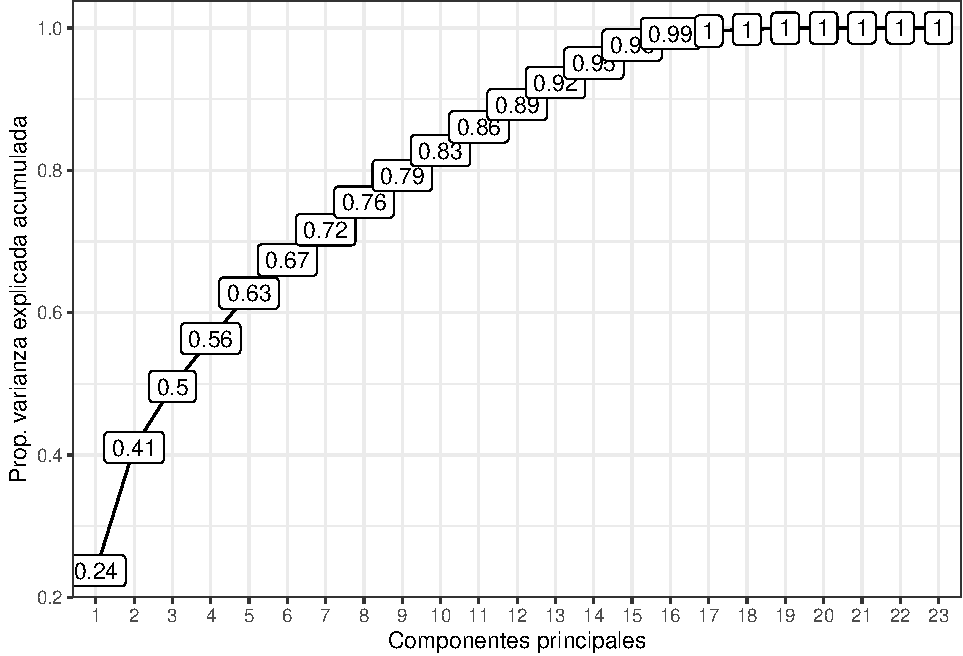
\includegraphics{00_pca_tsne_cluster_files/figure-latex/unnamed-chunk-7-1.pdf}

\begin{table}[!h]

\caption{\label{tab:loadings_pca_tablon}Loadings de PCA en Tablon}
\centering
\begin{tabular}[t]{lrrrr}
\toprule
\rowcolor{black}  \multicolumn{1}{c}{\textcolor{white}{\textbf{variable}}} & \multicolumn{1}{c}{\textcolor{white}{\textbf{PC1}}} & \multicolumn{1}{c}{\textcolor{white}{\textbf{PC2}}} & \multicolumn{1}{c}{\textcolor{white}{\textbf{PC3}}} & \multicolumn{1}{c}{\textcolor{white}{\textbf{PC4}}}\\
\midrule
\rowcolor{gray!6}  Turno\_Manana & 0.2813063 & -0.1375132 & 0.0171629 & 0.0891187\\
tipo\_de\_aprobacion\_libre & -0.0516192 & -0.2204644 & -0.1151088 & -0.3721061\\
\rowcolor{gray!6}  tipo\_de\_aprobacion\_cambio\_curso & 0.0985927 & -0.0960438 & 0.0259816 & -0.0003118\\
tipo\_de\_aprobacion\_promociono & 0.3581733 & 0.1308245 & -0.0808955 & 0.0804953\\
\rowcolor{gray!6}  edad\_al\_ingreso & -0.1269356 & 0.0733137 & -0.2349852 & -0.2976394\\
\addlinespace
tipo\_de\_aprobacion\_no\_firmo & 0.0156176 & -0.4488391 & -0.1126781 & -0.1126948\\
\rowcolor{gray!6}  ciclo\_lectivo\_de\_cursada & 0.1818683 & -0.0532719 & -0.1144249 & -0.0532596\\
tipo\_de\_aprobacion\_firmo & 0.3996032 & 0.0206986 & 0.0690403 & -0.0132481\\
\rowcolor{gray!6}  cant\_resursada\_regular & 0.0227835 & -0.3127946 & -0.4101361 & 0.3674317\\
cant\_recursada\_regular\_No\_Recurso & 0.3869691 & 0.1219610 & 0.0468956 & 0.0352279\\
\addlinespace
\rowcolor{gray!6}  cant\_recursada\_regular\_Recurso1vez & 0.1188652 & -0.2681558 & 0.0654967 & -0.1891977\\
cant\_recursada\_regular\_Recurso2vez & 0.0451665 & -0.2939066 & -0.0071695 & -0.1971879\\
\rowcolor{gray!6}  cant\_recursada\_regular\_Recurso3vez & 0.0120116 & -0.2503402 & -0.0867234 & -0.1612458\\
cant\_recursada\_regular\_Recurso4vez & 0.0044083 & -0.1971933 & -0.0845225 & -0.1281708\\
\rowcolor{gray!6}  cant\_recursada\_regular\_Recurso5vez & 0.0006389 & -0.1464459 & -0.1411299 & 0.0048529\\
\addlinespace
cant\_recursada\_regular\_RecursoNveces & -0.0021967 & -0.1955233 & -0.4257671 & 0.4879239\\
\rowcolor{gray!6}  Turno\_Tarde & 0.1153361 & -0.1754377 & 0.0127343 & 0.0859205\\
Turno\_Noche & 0.2032766 & -0.1098708 & -0.0798642 & -0.3755512\\
\rowcolor{gray!6}  Aprobado & 0.3918783 & 0.1006967 & -0.0242947 & -0.0374767\\
Promociono & 0.3589365 & 0.1289055 & -0.0812155 & 0.0798013\\
\addlinespace
\rowcolor{gray!6}  noAprobado & 0.2504186 & -0.1806504 & 0.2037648 & -0.0519875\\
Nota & -0.0001346 & 0.3003970 & -0.4732939 & -0.2012817\\
\rowcolor{gray!6}  Nota\_max\_prom & 0.0688392 & 0.2670847 & -0.4728596 & -0.2279385\\
\bottomrule
\end{tabular}
\end{table}

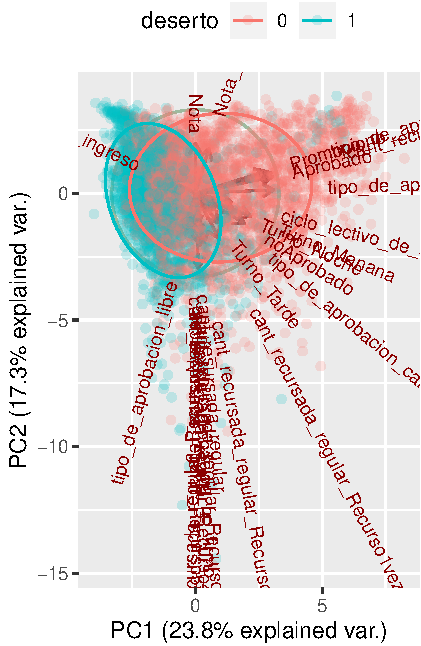
\includegraphics{00_pca_tsne_cluster_files/figure-latex/unnamed-chunk-9-1.pdf}

Se puede observar que si bien se puede reducir la cantidad de variables
predictoras y mantener una alta variabilidad de la información
explicada, los diagramas de biplot en este caso no nos servirían de
mucha ayuda ya que en las primeras 2 componentes solo se explica el 41\%
y en las primeras 4 componentes solo el 56\%. Además, los loadings de
dichos componentes no tienen una clara identificación de la proyección
que quieren significar, por lo que sería complicado explicar el modelo
que se queira desarrollar según estas nuevas variables.

\hypertarget{reducciuxf3n-por-t-sne}{%
\paragraph{Reducción por t-SNE}\label{reducciuxf3n-por-t-sne}}

Al igual que PCA, existen otro algoritmos que pueden realizar ruducción
de dimensionalidad. Unos de esos casos es el método no lineal
t-distributed stochastic neighbor embedding (t-SNE), que en ciertos
casos es ventajoso respecto a PCA que aplica reducción pero utilizando
combinaciones lineales de las variables originales.

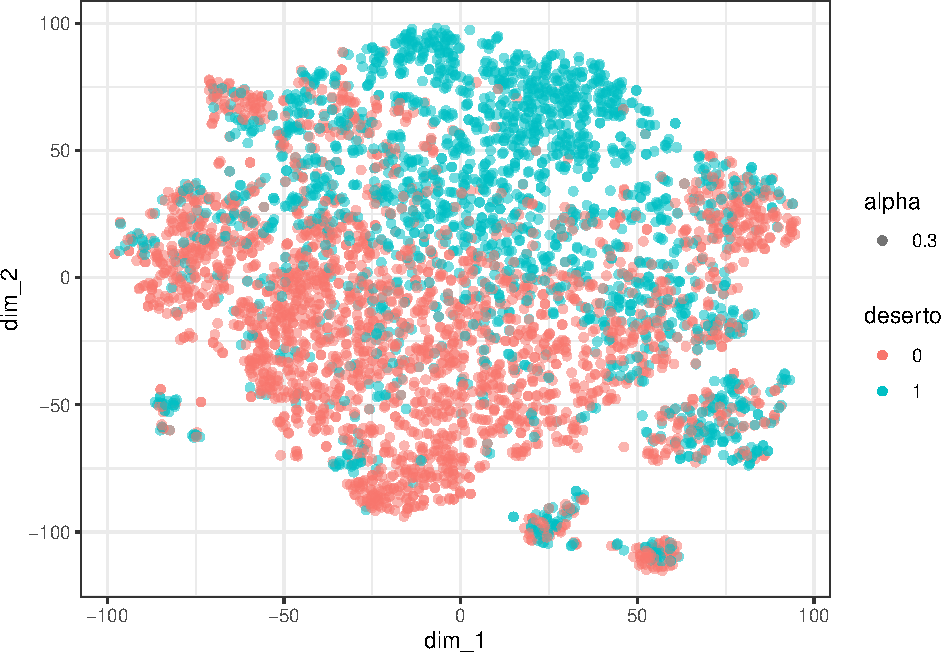
\includegraphics{00_pca_tsne_cluster_files/figure-latex/unnamed-chunk-11-1.pdf}

Utilizando el método T-SNE, si bien no se arman grupos bien definidos,
al identificar cada observación con un color en el gráfico según el
target puede observarse que están mas separadas y hay menos solapamiento
entre ellas que con el método PCA. Este resultado puede insinuar que es
posible clasificar un gran porcentaje de los casos correctamente.

\hypertarget{clusters}{%
\paragraph{Clusters}\label{clusters}}

Se utilizarán técnicas de clusters sobre la base del tablón y las
reducciones de dimensión calculadas anteriormente.

Criterio: * Como son solamente 2 las variables categóricas (EsTecnico y
sexo), en vez de calcular las distancias numéricas por un lado
(euclídea, manhattan, correlación, etc), las distancias categóricas por
otras (SMC, Jaccard, etc) y tratar de transformar esas matrices de
distancias en una nueva matriz unificada con criterios, se decide
transformar los datos categóricos en numéricos aprovechndo que ambos
campos tiene solamente 2 valores por lo que estarán en los extremos
tomando una normalización entre 0 y 1. En el caso de las observaciones
que con valor nulo en la variable EsTecnico, se imputará con el valor
0.5 (mitad entre extremos)

\begin{lstlisting}
## [1] 0.8893004
\end{lstlisting}

El estadístico de Hopkins sobre el tablon orifginal transformado las 2
variable cateóricas en numéricas da 0.8893004. Es un valor cercano a 1
por lo que tiene mucha tendencia a ser clusterizado.

\hypertarget{matriz-distancia-entre-variables}{%
\paragraph{Matriz distancia entre
variables}\label{matriz-distancia-entre-variables}}

Matriz

\hypertarget{estudio-del-nuxfamero-uxf3ptimo-de-clusters}{%
\paragraph{Estudio del número óptimo de
clusters}\label{estudio-del-nuxfamero-uxf3ptimo-de-clusters}}

Por la cantidad de datos que hay en el dataset y el poder computacional

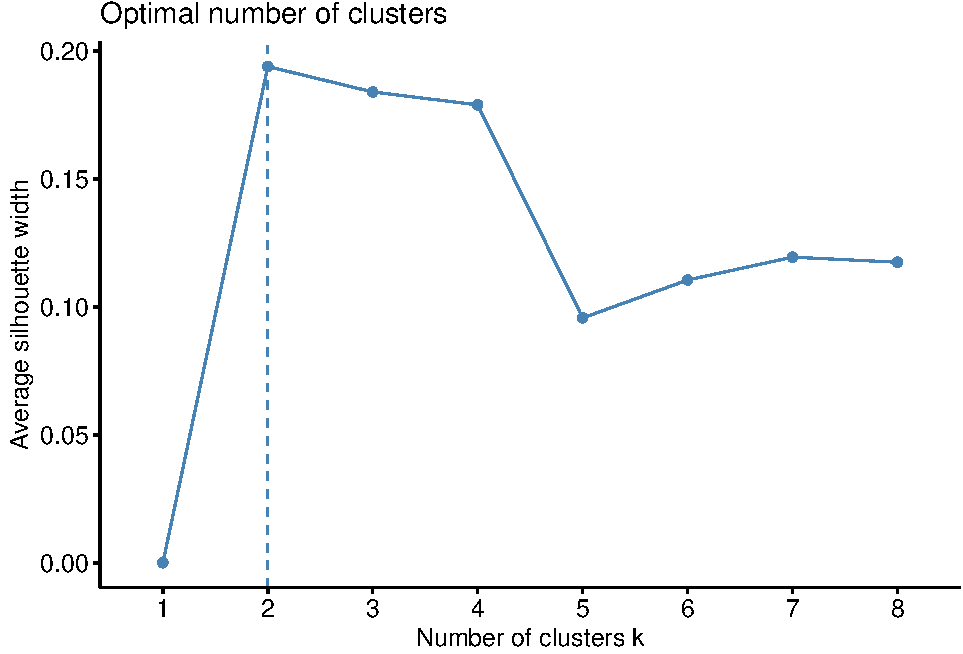
\includegraphics{00_pca_tsne_cluster_files/figure-latex/unnamed-chunk-15-1.pdf}
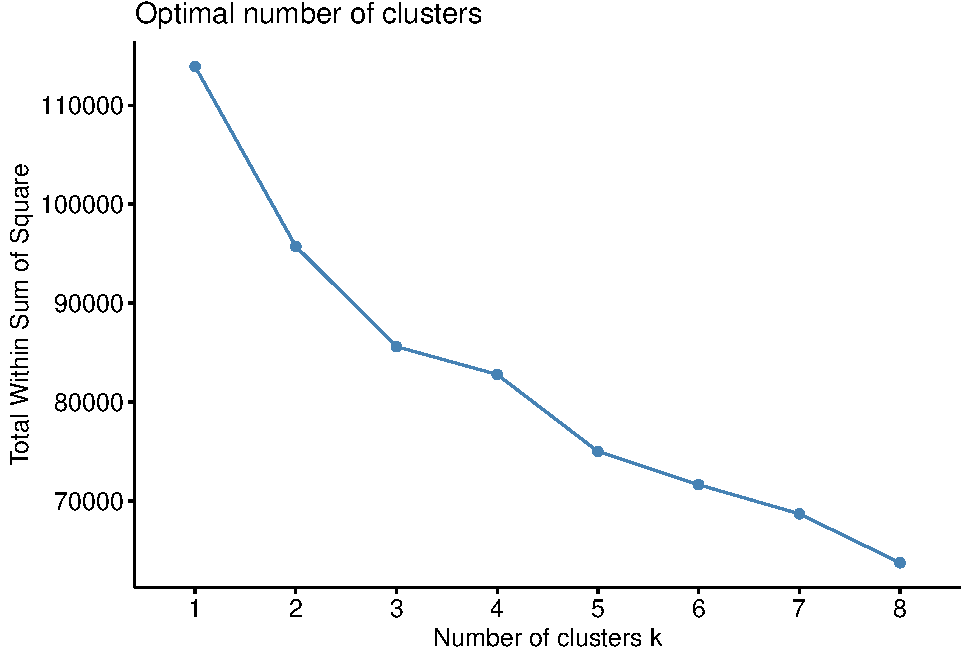
\includegraphics{00_pca_tsne_cluster_files/figure-latex/unnamed-chunk-15-2.pdf}

Verificación de las funciones anteriores de número óptio de clsuters
pero calculadas manualmente

\begin{lstlisting}
## 
## Clustering Methods:
##  kmeans hierarchical 
## 
## Cluster sizes:
##  2 3 4 5 
## 
## Validation Measures:
##                                    2         3         4         5
##                                                                   
## kmeans       Connectivity     0.0000    3.1667  730.2742 1316.3881
##              Dunn             0.4693    0.5735    0.0471    0.0345
##              Silhouette       0.5937    0.5336    0.2070    0.1796
## hierarchical Connectivity     3.1667    3.1667    9.2357   12.1647
##              Dunn             0.5713    0.5735    0.2744    0.2744
##              Silhouette       0.7329    0.5336    0.5198    0.4879
## 
## Optimal Scores:
## 
##              Score  Method       Clusters
## Connectivity 0.0000 kmeans       2       
## Dunn         0.5735 kmeans       3       
## Silhouette   0.7329 hierarchical 2
\end{lstlisting}

\begin{itemize}
\item
  Método Kmeans: Los resultados anteriores de validaciones internas,
  nuevamente nos da que la òptima solución son 2 clusters en las
  métricas de Siloutte y Connectivity mientras que para la métrica de
  Dunn el óptimo número de clusters sería 3.
\item
  Método Jerárquico: E esta validación se agregó el método jerárquico en
  el cual las métricas Connectivity y Dunn dan resultados iguales
  mientras que en silhouette es mejor el resultado con 2 clusters.
\end{itemize}

La conslución que podes sacar es que pareciera ser que la mejor solución
es hacer clusters de 2 grupos ya sea por el método Kmeans o Jerárquico.

\hypertarget{cluster-kmeans}{%
\paragraph{Cluster Kmeans}\label{cluster-kmeans}}

Tomando como referencia las validaciones anteriores, se realizará un
cluster kmeans con 2 centroides. Este método se repetirá 25 veces
distintas se elegirá el mejor.

\begin{lstlisting}
##   cluster size ave.sil.width
## 1       1 1275          0.19
## 2       2 3283          0.20
\end{lstlisting}

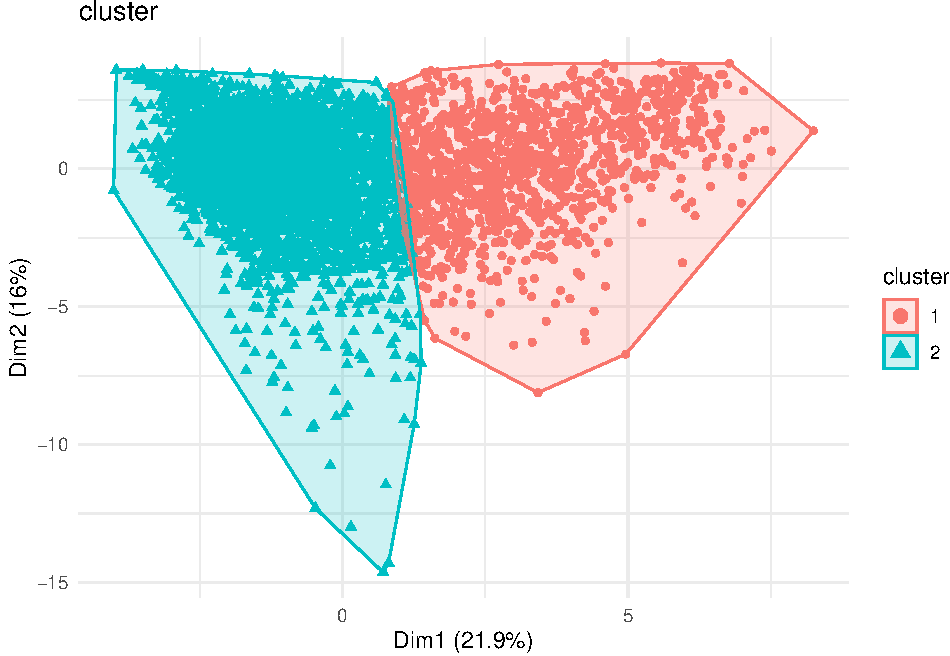
\includegraphics{00_pca_tsne_cluster_files/figure-latex/unnamed-chunk-18-1.pdf}
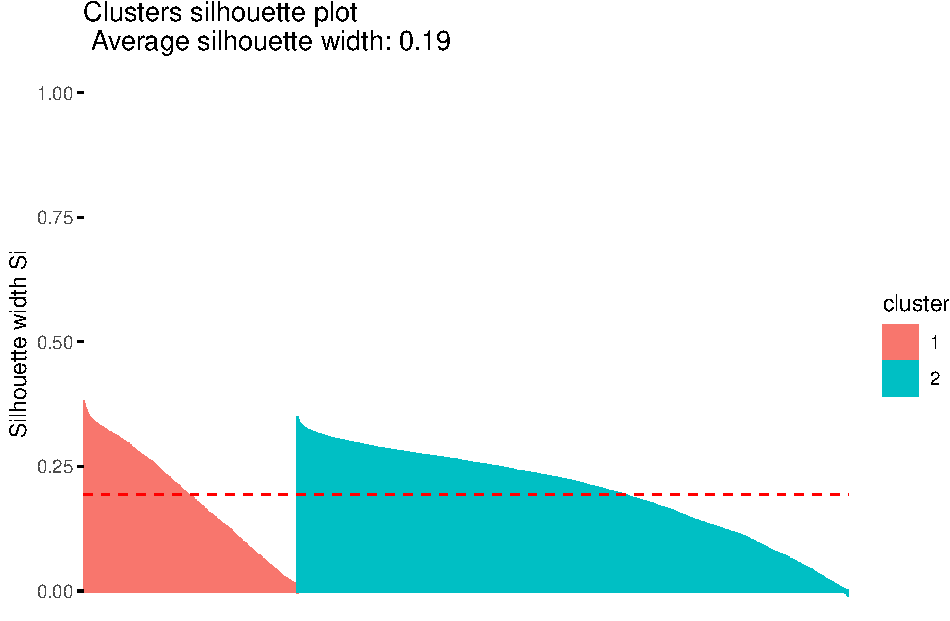
\includegraphics{00_pca_tsne_cluster_files/figure-latex/unnamed-chunk-18-2.pdf}

El cluster parece ser muy bueno. Por lo tanto el próximo paso es saber
en que cluster cae cada observación según su target

\begin{table}[!h]

\caption{\label{tab:kmeans_2_resumen}Resumen composición de cluster Kmeans según clase desertor}
\centering
\begin{tabular}[t]{rrrrrr}
\toprule
\rowcolor{black}  \multicolumn{1}{c}{\textcolor{white}{\textbf{grupo}}} & \multicolumn{1}{c}{\textcolor{white}{\textbf{cant\_integrantes}}} & \multicolumn{1}{c}{\textcolor{white}{\textbf{cant\_desertores}}} & \multicolumn{1}{c}{\textcolor{white}{\textbf{cant\_desertores\_pct}}} & \multicolumn{1}{c}{\textcolor{white}{\textbf{cant\_no\_desertores}}} & \multicolumn{1}{c}{\textcolor{white}{\textbf{cant\_no\_desertores\_pct}}}\\
\midrule
\rowcolor{gray!6}  1 & 1275 & 142 & 11.13725 & 1133 & 88.86275\\
2 & 3283 & 1858 & 56.59458 & 1425 & 43.40542\\
\bottomrule
\end{tabular}
\end{table}

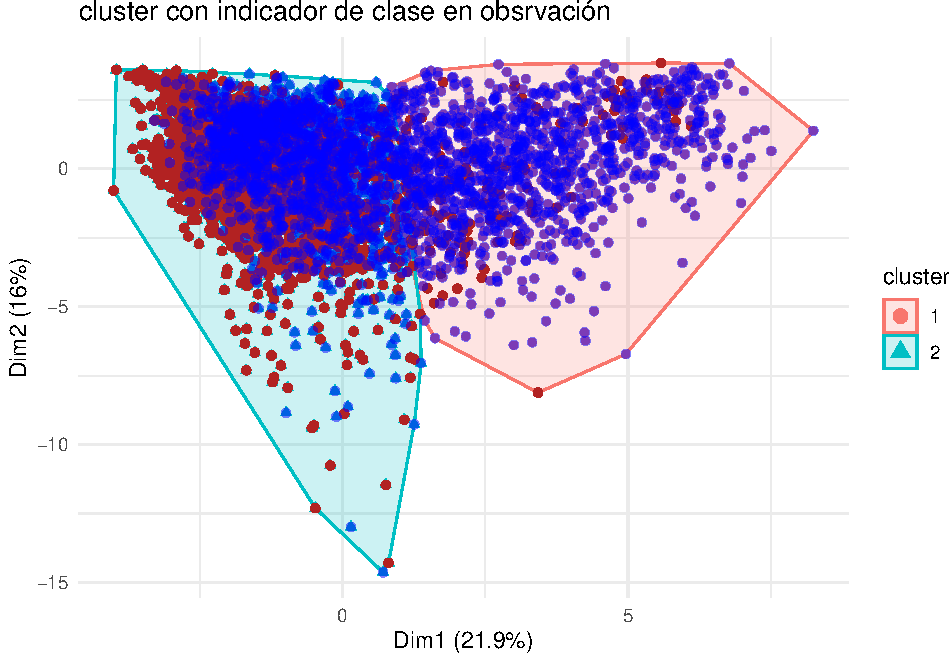
\includegraphics{00_pca_tsne_cluster_files/figure-latex/unnamed-chunk-21-1.pdf}

Puede observarse que un grupo contiene solamente un 11,13\% de datos
erroneos, pero el otro grupo està muy balanceado. Por lo tanto, el
cluster de 2 grupos a pesar de que tenga muy buenos valores en las
validaciones realizadas, al verificar con el target real donde queda
cada obsevación no es un buen resultado. En el gráfico se observa lo
expresado en la tabla.

\hypertarget{cluster-jeruxe1rquico}{%
\paragraph{cluster jerárquico}\label{cluster-jeruxe1rquico}}

Siguiendo lo sugerido se realiza el cluster jerárquico. Es de destacar
que esta vez no puede mostrarse el dendograma completo ya que la
cantidad de observaciones son muchas. Por lo cual, según lo sugerido en
las validaciones, se hará el cote en 2 grupos y se verificará según la
clase si la composición de los grupos se relaciona bien con e target.

Se realizan 4 cluster jerarquicos, cada uno utilizando las medidas de
distancias ``complete'', ``average'', ``single'', ``ward''.

\begin{table}[!h]

\caption{\label{tab:tabla_cophenetic_jerarquico}Coef. cophenetic por cada tipo de cluster jerárquico}
\centering
\begin{tabular}[t]{lr}
\toprule
\rowcolor{black}  \multicolumn{1}{c}{\textcolor{white}{\textbf{metodo}}} & \multicolumn{1}{c}{\textcolor{white}{\textbf{coeficiente\_cofenetico}}}\\
\midrule
\rowcolor{gray!6}  complete & 0.7199776\\
average & 0.8142721\\
\rowcolor{gray!6}  single & 0.7217462\\
ward & 0.3765082\\
\bottomrule
\end{tabular}
\end{table}

El tipo de distancia del cluster jerárquico que arroja el mayor
coeficiente cophenetico es ``average'' con un valor de 0.8142721.

\begin{table}[!h]

\caption{\label{tab:tabla_jerarquico_composicion}Composición de clusters según la clase deserto}
\centering
\resizebox{\linewidth}{!}{
\begin{tabular}[t]{rrrrrr}
\toprule
\rowcolor{black}  \multicolumn{1}{c}{\textcolor{white}{\textbf{grupo}}} & \multicolumn{1}{c}{\textcolor{white}{\textbf{cant\_integrantes}}} & \multicolumn{1}{c}{\textcolor{white}{\textbf{cant\_desertores}}} & \multicolumn{1}{c}{\textcolor{white}{\textbf{cant\_desertores\_pct}}} & \multicolumn{1}{c}{\textcolor{white}{\textbf{cant\_no\_desertores}}} & \multicolumn{1}{c}{\textcolor{white}{\textbf{cant\_no\_desertores\_pct}}}\\
\midrule
\rowcolor{gray!6}  1 & 4550 & 1996 & 43.86813 & 2554 & 56.13187\\
2 & 8 & 4 & 50.00000 & 4 & 50.00000\\
\bottomrule
\end{tabular}}
\end{table}

se puede observar que forma un grupo muy numeroso y otro muy chico y
ambos estan muy mezclados en función el target. Por lo tanto, el método
jerárquico no es adecuado.

\hypertarget{extensiuxf3n-de-clusters}{%
\paragraph{Extensión de Clusters}\label{extensiuxf3n-de-clusters}}

A pesar del estudio de validaciones y resultados anteriormente,
igualmente queremos ver cuales son los resultados que nos arrojan hacer
mas de 2 clusters. Como los resultados los referenciamos al target,
campo que no se incluye en los datos para ahcer cluster al ser no
supervisado, podría darse el caso de que en la situación real otro
número de cluster sea óptima a la que arrojan las validaciones
matemáticas.

\begin{table}[!h]

\caption{\label{tab:tabla_muchos_clusters}Resumen por tipo de cluster, cantidad de clusters y la composición de cada uno según la clase deserto}
\centering
\resizebox{\linewidth}{!}{
\begin{tabular}[t]{lrrrrrrrrrrr}
\toprule
\rowcolor{black}  \multicolumn{1}{c}{\textcolor{white}{\textbf{metodo}}} & \multicolumn{1}{c}{\textcolor{white}{\textbf{numero\_clusters}}} & \multicolumn{1}{c}{\textcolor{white}{\textbf{1\_N}}} & \multicolumn{1}{c}{\textcolor{white}{\textbf{1\_S}}} & \multicolumn{1}{c}{\textcolor{white}{\textbf{2\_N}}} & \multicolumn{1}{c}{\textcolor{white}{\textbf{2\_S}}} & \multicolumn{1}{c}{\textcolor{white}{\textbf{3\_N}}} & \multicolumn{1}{c}{\textcolor{white}{\textbf{3\_S}}} & \multicolumn{1}{c}{\textcolor{white}{\textbf{4\_N}}} & \multicolumn{1}{c}{\textcolor{white}{\textbf{4\_S}}} & \multicolumn{1}{c}{\textcolor{white}{\textbf{5\_N}}} & \multicolumn{1}{c}{\textcolor{white}{\textbf{5\_S}}}\\
\midrule
\rowcolor{gray!6}  jerarquico & 2 & 2554 & 1996 & 4 & 4 & NA & NA & NA & NA & NA & NA\\
jerarquico & 3 & 2544 & 1972 & 10 & 24 & 4 & 4 & NA & NA & NA & NA\\
\rowcolor{gray!6}  jerarquico & 4 & 2544 & 1970 & NA & 2 & 10 & 24 & 4 & 4 & NA & NA\\
jerarquico & 5 & 2543 & 1970 & NA & 2 & 10 & 24 & 1 & NA & 4 & 4\\
\rowcolor{gray!6}  kmeans & 2 & 1133 & 142 & 1425 & 1858 & NA & NA & NA & NA & NA & NA\\
\addlinespace
kmeans & 3 & 878 & 82 & 611 & 604 & 1069 & 1314 & NA & NA & NA & NA\\
\rowcolor{gray!6}  kmeans & 4 & 1028 & 1252 & 842 & 73 & 14 & 28 & 674 & 647 & NA & NA\\
kmeans & 5 & 725 & 576 & 400 & 837 & 606 & 487 & 14 & 28 & 813 & 72\\
\bottomrule
\end{tabular}}
\end{table}

A continuación mostramos un grafico resumen sobre

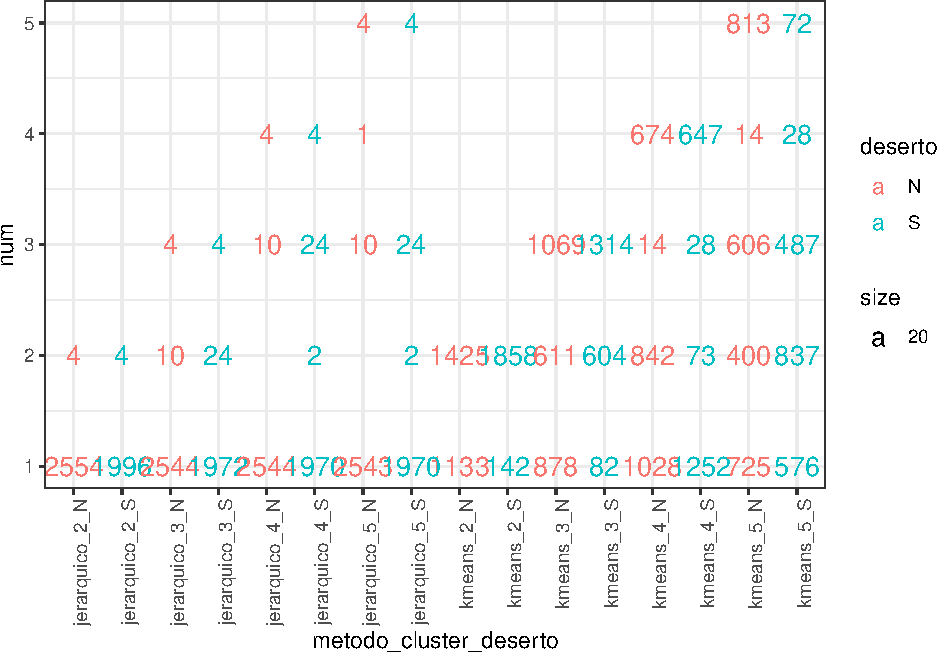
\includegraphics{00_pca_tsne_cluster_files/figure-latex/unnamed-chunk-25-1.pdf}

La figura muestra la misma información que el cuadro anterior. En el eje
x indica que tipo de cluster es, cuantos clusters y la clase deserto
(``S'' y ``N''). En el eje y se indica el numero de cluster, por lo que
los cluster armados solo con 2 clusters, habrá información únicamente
hasta esa altura. Por ejemplo, para el el caso de aplciar un método
jerárquico de 2 clusters podemos observar que en el primer cluster
tenemos 2554 casos Negatigos y 1996 casos positivos, mientras que el
cluster número 2 esta conformado de 4 casos negativos y 4 casos
positivos.

\end{document}
